\chapter{Covariant Electromagnetism}\label{ch:b3:covariant-electromagnetism}

A copper wire carries ten amperes. Its electrons drift at a tenth of
a millimetre per second --- slower than a snail --- and the wire is
electrically neutral to fantastic precision. Yet a charge moving
alongside feels a measurable pull. Viewed from that charge's own
frame, the ``magnetic'' explanation evaporates: the charge is at
rest, and a resting charge feels no magnetic force at all. What pulls
it, in that frame, is an \emph{electric} field --- conjured by
relativity itself, because \omterm{prop:b3:relativistic-kinematics:contraction}{length contraction} unbalances, by one part
in $10^{24}$, the two streams of charge in the wire. Magnetism is
electricity seen from a moving seat. This chapter rewrites the
electromagnetism of the Year 2 volume in the language of the previous
three: \omterm{def:b3:covariant-electromagnetism:fourvector}{four-vectors} for charge and potential, one antisymmetric
tensor holding $\vect E$ and $\vect B$ together, Maxwell's four
equations collapsing into two lines that read the same in every
\omterm{thm:b3:relativistic-kinematics:postulates}{inertial frame}. Beyond elegance, the payoff is working physics: how
fields transform, why a fast charge's field flattens into a pancake,
and why the light of a relativistic electron sweeps forward like a
headlight --- the principle of the synchrotron light sources that
X-ray proteins and batteries today.

\section{Four-vectors for charge and current}

\begin{definition}[Four-vectors]\label{def:b3:covariant-electromagnetism:fourvector}
\index{four-vector}
A \emph{four-vector} is a quadruple $a^\mu = (a^0, \vect a)$, $\mu =
0, 1, 2, 3$, whose components mix under a boost exactly as $(ct,
\vect r)$ do:
\[
a'^0 = \gamma(a^0 - \beta a^1) , \qquad
a'^1 = \gamma(a^1 - \beta a^0) , \qquad
a'^{2,3} = a^{2,3}
\]
for a boost at $\beta c$ along $x$. Any two four-vectors give the
invariant scalar product $a\cdot b = a^0b^0 - \vect a\cdot\vect b$,
the same number in every frame --- the pattern behind $c^2t^2 - x^2$
and $E^2 - p^2c^2$. Position $(ct, \vect r)$ and \omterm{def:b3:relativistic-dynamics:four-momentum}{four-momentum}
$(E/c, \vect p)$ are the two we have; electromagnetism now supplies
three more: current, potential, and wave-vector.
\end{definition}

\begin{proposition}[The four-current and charge conservation]\label{prop:b3:covariant-electromagnetism:fourcurrent}
\index{four-current}
Charge density $\rho$ and current density $\vect\jmath$ form the
four-current
\[
J^\mu = (\rho c,\ \vect\jmath\,) :
\]
a cloud of charge of proper density $\rho_0$ moving at $\vect u$ has
$J^\mu = \rho_0\gamma_u(c, \vect u)$ --- density grows by $\gamma_u$
because the cloud's volume contracts, while the charge itself is
invariant (a decisive experimental fact: atoms with fast inner
electrons stay exactly neutral). Charge conservation is the
invariant statement
\[
\frac{\partial(\rho c)}{\partial(ct)} +
\operatorname{div}\vect\jmath = 0 ,
\]
the continuity equation of the Year 2 volume, now visibly the same
law for all observers.
\end{proposition}

\begin{proof}[Partial proof]
The moving cloud: a box of proper volume $V_0$ holds charge $\rho_0
V_0$; in the lab the box is contracted to $V_0/\gamma_u$, so $\rho =
\gamma_u\rho_0$, and $\vect\jmath = \rho\vect u$ by definition of a
current density. That $(\rho c, \vect\jmath)$ then transforms as a
\omterm{def:b3:covariant-electromagnetism:fourvector}{four-vector} follows because it equals $\rho_0/c$ times the
four-velocity $\gamma_u(c, \vect u)$, itself \omterm{def:b3:covariant-electromagnetism:fourvector}{four-vector} by
construction. Invariance of charge is an experimental input.
\end{proof}

\section{One tensor for both fields}

\begin{definition}[Four-potential and field tensor]\label{def:b3:covariant-electromagnetism:tensor}
\index{four-potential}\index{field tensor}
The potentials of the Year 2 volume assemble into the four-potential
\[
A^\mu = \Big(\frac{V}{c},\ \vect A\Big) ,
\]
and the measurable fields $\vect E = -\vect\nabla V -
\partial_t\vect A$, $\vect B = \operatorname{\vect{curl}}\vect A$ are
the six independent components of one antisymmetric array, the
\emph{electromagnetic field tensor}
\[
F^{\mu\nu} =
\begin{pmatrix}
0 & -E_x/c & -E_y/c & -E_z/c\\
E_x/c & 0 & -B_z & B_y\\
E_y/c & B_z & 0 & -B_x\\
E_z/c & -B_y & B_x & 0
\end{pmatrix} .
\]
$\vect E$ and $\vect B$ are not two fields but six faces of one
object; which face an observer calls ``electric'' depends on the
observer's motion.
\end{definition}

\begin{theorem}[Maxwell, covariantly]\label{thm:b3:covariant-electromagnetism:maxwell}
\index{Maxwell's equations!covariant form}
The four Maxwell equations of the Year 2 volume are the component
form of two frame-independent statements: the sourced pair
(Gauss and Ampère--Maxwell) is
\[
\sum_\mu \partial_\mu F^{\mu\nu} = \mu_0\,J^\nu ,
\]
and the sourceless pair (no monopoles, Faraday) is the identity
guaranteeing that $F$ derives from a \omterm{def:b3:covariant-electromagnetism:tensor}{four-potential}. The Lorentz
force is $\dd p^\mu/\dd\tau = qF^{\mu\nu}u_\nu$ --- force law,
magnetic included, in one line. Because both sides of each equation
transform identically, \emph{Maxwell's theory needs no correction to
be relativistic}: it was relativity's first finished piece, born
1865.
\end{theorem}

\begin{proof}[Partial proof]
Expand the $\nu = 0$ component: $\sum_i\partial_i(E_i/c) =
\mu_0\rho c$, i.e.\ $\operatorname{div}\vect E = \rho/\varepsilon_0$
(using $c^2 = 1/\mu_0\varepsilon_0$). The $\nu = 1$ component
collects $-\partial_t(E_x/c^2) + (\partial_yB_z - \partial_zB_y)
= \mu_0 j_x$: the $x$ component of Ampère--Maxwell. The other
components repeat the pattern; the sourceless pair is the equality of
crossed second derivatives of $A^\mu$ (checked in
\cref{exo:b3:covariant-electromagnetism:3}). That $F^{\mu\nu}$
transforms as a (two-index) tensor --- each index like a \omterm{def:b3:covariant-electromagnetism:fourvector}{four-vector}
--- is admitted; its consequences are the next proposition.
\end{proof}

\section{How the fields transform}

\begin{proposition}[Field transformation]\label{prop:b3:covariant-electromagnetism:transform}
\index{field transformation}
For a boost at velocity $\vect v = v\,\vect e_x$: the components
\emph{along} the motion are untouched, the transverse ones mix,
\[
E'_x = E_x , \qquad
E'_y = \gamma(E_y - vB_z) , \qquad
E'_z = \gamma(E_z + vB_y) ,
\]
\[
B'_x = B_x , \qquad
B'_y = \gamma\Big(B_y + \frac{v}{c^2}E_z\Big) , \qquad
B'_z = \gamma\Big(B_z - \frac{v}{c^2}E_y\Big) .
\]
Compactly, transverse to the boost: $\vect E' = \gamma(\vect E +
\vect v\wedge\vect B)_\perp$ and $\vect B' = \gamma(\vect B - \vect
v\wedge\vect E/c^2)_\perp$. A pure $\vect B$ in one frame is $\vect
E$ and $\vect B$ in another: the fields are one phenomenon.
\end{proposition}
\admitted

\begin{example}[Magnetism from a neutral wire]\label{ex:b3:covariant-electromagnetism:wire}
A neutral wire carries current: positive lattice at rest, electrons
drifting. For a test charge moving alongside, boost to its frame: the
two charge streams contract \emph{differently} (they have different
velocities), the wire acquires the net line charge $\lambda' =
-\gamma vI/c^2$, and its radial electric field pulls the charge with
exactly the force the lab called $q\vect v\wedge\vect B$. Magnetism
is what the second-order term $v u/c^2$ of relativity looks like when
$10^{28}$ elementary charges per metre conspire: each effect is
fantastically small, but the wire is neutral to even greater
precision, so the tiny imbalance is the whole story
(\cref{pb:b3:covariant-electromagnetism:1}).
\end{example}

\begin{omfigure}
\begin{tikzpicture}[font=\small, >=Stealth]
  % lab frame
  \begin{scope}
    \draw[thick, fill=omExo!10] (-0.2,0) rectangle (5.4,0.75);
    \foreach \x in {0.3,1.3,2.3,3.3,4.3} \node[omThm] at (\x,0.52) {$\oplus$};
    \foreach \x in {0.8,1.8,2.8,3.8,4.8} {\node[omDef] at (\x,0.22) {$\ominus$};
      \draw[->, omDef] (\x+0.16,0.22) -- (\x+0.42,0.22);}
    \fill[omProp] (2.6,-1.15) circle (2.6pt);
    \draw[->, omProp, thick] (2.75,-1.15) -- (3.55,-1.15);
    \node[anchor=west] at (3.65,-1.15) {$q$, speed $v$};
    \draw[->, very thick] (2.6,-0.95) -- (2.6,-0.35);
    \node[anchor=west, font=\footnotesize] at (2.7,-0.62) {$q\vect v\wedge\vect B$};
    \node at (2.6,1.35) {lab: wire neutral, force magnetic};
  \end{scope}
  % charge frame
  \begin{scope}[xshift=7.8cm]
    \draw[thick, fill=omExo!10] (-0.2,0) rectangle (5.4,0.75);
    \foreach \x in {0.25,1.15,2.05,2.95,3.85,4.75} {\node[omThm] at (\x,0.52) {$\oplus$};
      \draw[->, omThm] (\x-0.14,0.72) -- (\x-0.4,0.72);}
    \foreach \x in {0.7,1.9,3.1,4.3} \node[omDef] at (\x,0.22) {$\ominus$};
    \fill[omProp] (2.6,-1.15) circle (2.6pt);
    \node[anchor=west] at (2.75,-1.35) {$q$ at rest};
    \draw[->, very thick] (2.6,-0.95) -- (2.6,-0.35);
    \node[anchor=west, font=\footnotesize] at (2.7,-0.62) {$q\vect E'$};
    \node at (2.6,1.35) {charge frame: wire charged, force electric};
  \end{scope}
\end{tikzpicture}

{\small One force, two accountings. Lab: the neutral wire's current
makes $\vect B$, the moving charge feels $q\vect v\wedge\vect B$.
Charge's frame: the positive lattice now moves and contracts, the
electrons (slower there) spread out; the wire is net charged and its
$\vect E'$ does the pulling. Same experiment, same outcome.}
\end{omfigure}

\begin{example}[The pancaked field of a fast charge]\label{ex:b3:covariant-electromagnetism:pancake}
Transform the Coulomb field of a charge into the frame where it moves
at $\gamma \gg 1$: the longitudinal field is unchanged while the
transverse one is multiplied by $\gamma$. The once-spherical field
flattens into a disc of opening angle $\sim 1/\gamma$ around the
plane through the charge --- accompanied, transverse to the motion,
by a magnetic ring $B' = vE'/c^2$. To a stationary observer the
passage of an LHC proton ($\gamma \approx 7000$) is a
sub-picosecond slap of nearly-crossed $\vect E$ and $\vect B$: almost
a pulse of light --- the reason fast beams talk to matter the way
photons do.
\end{example}

\begin{omfigure}
\begin{tikzpicture}[font=\small, >=Stealth]
  % static charge
  \begin{scope}
    \fill[omThm] (0,0) circle (2.6pt);
    \foreach \a in {0,30,...,330} \draw[->, omDef] (\a:0.25) -- (\a:1.75);
    \node at (0,-2.5) {at rest: isotropic Coulomb field};
  \end{scope}
  % moving charge
  \begin{scope}[xshift=8.0cm]
    \fill[omThm] (0,0) circle (2.6pt);
    \draw[->, very thick] (0.3,-2.1) -- (1.5,-2.1) node[right] {$v \approx c$};
    \foreach \a/\l in {90/1.95, 75/1.5, 105/1.5, 60/0.85, 120/0.85,
                       270/1.95, 255/1.5, 285/1.5, 240/0.85, 300/0.85,
                       0/0.35, 180/0.35, 30/0.45, 150/0.45, 210/0.45, 330/0.45}
      \draw[->, omDef] (\a:0.25) -- (\a:\l);
    \node at (0,-2.5) {};
    \node at (0.3,-2.65) {};
    \node at (0,-2.9) {};
  \end{scope}
  \node at (8.0,-2.5) {moving: field pancaked into $\sim 1/\gamma$};
\end{tikzpicture}

{\small The electric field of a point charge, at rest and at high
speed: boosting multiplies the transverse components by $\gamma$ and
leaves the longitudinal ones alone, squeezing the field into a disc
perpendicular to the motion.}
\end{omfigure}

\section{Invariants, light, and the headlight effect}

\begin{proposition}[The two field invariants]\label{prop:b3:covariant-electromagnetism:invariants}
\index{field invariants}
From $F^{\mu\nu}$ one can build exactly two independent scalars:
\[
E^2 - c^2B^2
\qquad\text{and}\qquad
\vect E\cdot\vect B ,
\]
the same in every \omterm{thm:b3:relativistic-kinematics:postulates}{inertial frame}. Consequences: if $E > cB$ somewhere
(with $\vect E\cdot\vect B = 0$), some frame sees a pure electric
field there; if $E < cB$, some frame sees pure magnetic; and a plane
light wave, with $E = cB$ and $\vect E\perp\vect B$, has \emph{both}
invariants zero --- it is light in every frame: no boost can turn it
into a static field, only redshift it. One cannot catch up with a
light wave; Einstein's teenage question answers itself in two
invariants.
\end{proposition}

\begin{proof}[Partial proof]
Check invariance under the standard boost by direct substitution of
\cref{prop:b3:covariant-electromagnetism:transform}
(\cref{exo:b3:covariant-electromagnetism:6}); that no third
independent invariant exists is admitted. For the wave: $E = cB$ and
orthogonality give both zero; a frame with a static field would need
a nonzero invariant.
\end{proof}

\begin{proposition}[Four-wave-vector, Doppler and aberration]\label{prop:b3:covariant-electromagnetism:wavevector}
\index{aberration}\index{headlight effect}
A plane wave's frequency and direction form the null \omterm{def:b3:covariant-electromagnetism:fourvector}{four-vector}
$k^\mu = (\omega/c, \vect k)$, $\|\vect k\| = \omega/c$. Transforming
it gives at once the relativistic Doppler formula of
\cref{ch:b3:relativistic-kinematics} and the \emph{aberration} of
directions:
\[
\cos\theta' = \frac{\cos\theta - \beta}{1 - \beta\cos\theta} .
\]
Read backwards, a source radiating isotropically in its rest frame
beams, in the lab, half its light into the forward cone $\theta
\lesssim 1/\gamma$: the \emph{\omterm{prop:b3:covariant-electromagnetism:wavevector}{headlight effect}}. An electron circling
at $\gamma \sim 10^4$ in a storage ring sweeps a
$\qty{0.1}{mrad}$ searchlight of X-rays around the ring --- the
synchrotron light that fills protein-crystallography beamlines.
\end{proposition}

\begin{proof}[Partial proof]
The phase $\omega t - \vect k\cdot\vect r = k^\mu x_\mu$ counts wave
crests passing events --- an invariant --- so $k^\mu$ must transform
as a \omterm{def:b3:covariant-electromagnetism:fourvector}{four-vector}. Apply the boost to $(\omega/c, k\cos\theta,
k\sin\theta, 0)$: the time component gives Doppler, the ratio of
spatial components the aberration formula. Setting $\theta' =
90^\circ$ (the sideways ray of the source frame): $\cos\theta =
\beta$, i.e.\ $\theta \approx 1/\gamma$ for $\gamma \gg 1$ --- half
the sphere folds into the forward cone.
\end{proof}

\begin{omfigure}
\begin{tikzpicture}[font=\small, >=Stealth]
  % isotropic source
  \begin{scope}
    \fill[omThm] (0,0) circle (2.4pt);
    \foreach \a in {0,45,...,315} \draw[->, omExo] (\a:0.3) -- (\a:1.5);
    \node at (0,-2.2) {rest frame: isotropic};
  \end{scope}
  % beamed
  \begin{scope}[xshift=7.6cm]
    \fill[omThm] (0,0) circle (2.4pt);
    \draw[->, thick] (-1.9,0) -- (-0.6,0);
    \node at (-2.35,0) {$v$};
    \draw[->, omExo] (0.3,0.06) -- (2.6,0.55);
    \draw[->, omExo] (0.3,-0.06) -- (2.6,-0.55);
    \draw[->, omExo, very thick] (0.3,0) -- (2.9,0);
    \draw[->, omExo] (0.25,0.16) -- (1.5,1.0);
    \draw[->, omExo] (0.25,-0.16) -- (1.5,-1.0);
    \draw[->, omExo] (-0.1,0.28) -- (-0.5,1.0);
    \draw[->, omExo] (-0.1,-0.28) -- (-0.5,-1.0);
    \draw[dashed] (0,0) -- (3.1,0.85);
    \draw[dashed] (0,0) -- (3.1,-0.85);
    \node[anchor=west, font=\footnotesize] at (3.0,0.5) {$\sim 1/\gamma$};
    \node at (0.9,-2.2) {lab: a forward headlight};
  \end{scope}
\end{tikzpicture}

{\small Aberration folds the radiation of a fast source into a
forward cone of half-angle $\sim 1/\gamma$: the \omterm{prop:b3:covariant-electromagnetism:wavevector}{headlight effect}, and
the working principle of synchrotron light sources.}
\end{omfigure}

\begin{method}[Working covariantly]\label{met:b3:covariant-electromagnetism:method}
(1) Identify the \omterm{def:b3:covariant-electromagnetism:fourvector}{four-vectors} in play ($x^\mu$, $P^\mu$, $J^\mu$,
$A^\mu$, $k^\mu$) and prefer their invariant products to components.
(2) To transform fields, split into components along and transverse
to the boost and apply
\cref{prop:b3:covariant-electromagnetism:transform}. (3) Check the
two invariants before and after --- the fastest error detector in the
subject. (4) When a magnetic problem looks mysterious, ride with the
charge: in its frame only $\vect E'$ acts. (5) Trust Maxwell: the
equations never need relativistic ``corrections'', only relativistic
reading.
\end{method}

\begin{omfigure}
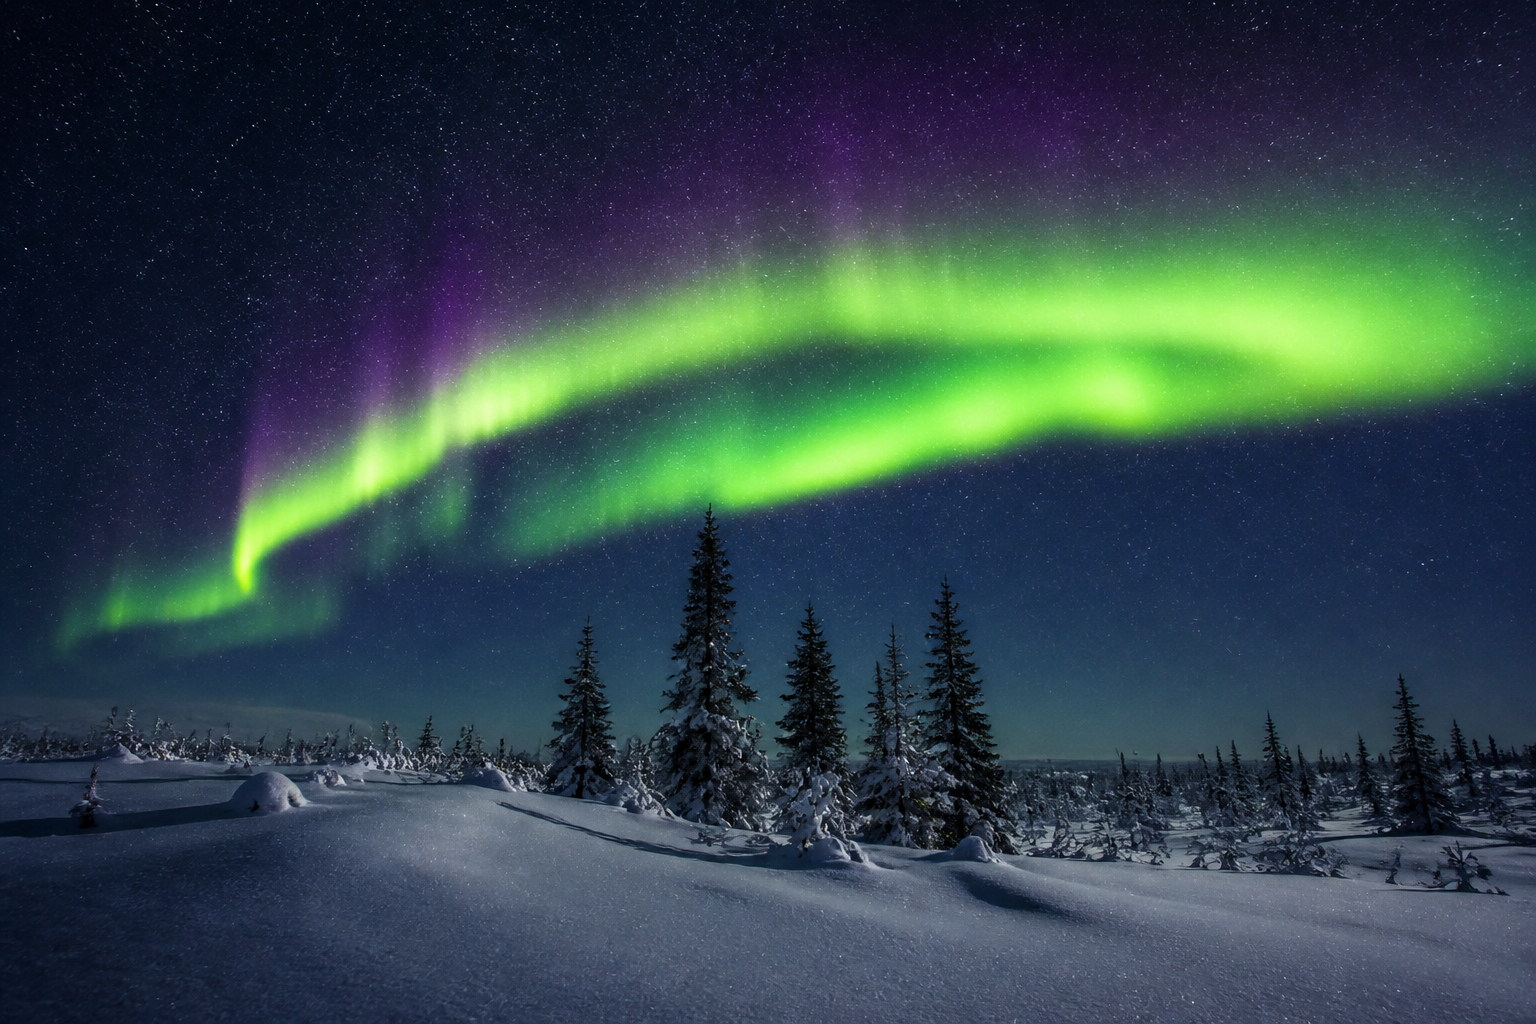
\includegraphics[width=0.58\linewidth]{images/book5/ai/b5-24-aurora-arc.png}

{\small An aurora: solar-wind charges steered by the Earth's magnetic field into the polar atmosphere. What one observer calls magnetic steering, another calls electric acceleration --- the fields mix under the transformations of this chapter.}
\end{omfigure}

\section{Exercises}

\begin{exercise}[$\star$]\label{exo:b3:covariant-electromagnetism:1}
(a) Boost $a^\mu = (5, 3, 0, 0)$ (units of some $a_0$) by $\beta =
0.6$: compute $a'^\mu$ and check $a\cdot a$ is unchanged. (b) Show
that the sum of two \omterm{def:b3:covariant-electromagnetism:fourvector}{four-vectors} is a \omterm{def:b3:covariant-electromagnetism:fourvector}{four-vector}. (c) Is $(c,
\vect v)$ of a particle a \omterm{def:b3:covariant-electromagnetism:fourvector}{four-vector}? And $\gamma(c, \vect v)$? (d)
Why is ``the electric field'' alone not part of any \omterm{def:b3:covariant-electromagnetism:fourvector}{four-vector}?
\end{exercise}

\begin{exercise}[$\star$]\label{exo:b3:covariant-electromagnetism:2}
A copper wire of section \qty{1.0}{mm^2} carries \qty{10}{A};
conduction-electron density $n = \qty{8.5e28}{m^{-3}}$. (a) Compute
the drift speed. (b) Write $J^\mu$ for the electron fluid and for the
lattice. (c) Check the continuity equation for each. (d) The wire is
neutral: what is $J^\mu$ for the whole wire, and which component
survives?
\end{exercise}

\begin{exercise}[$\star$]\label{exo:b3:covariant-electromagnetism:3}
(a) From the matrix of $F^{\mu\nu}$, read off which components give
$E_y$ and $B_x$. (b) Write $F^{\mu\nu}$ for a pure uniform field
$\vect B = B\vect e_z$, and for the field of a plane wave
($\vect E = E\vect e_y$, $\vect B = (E/c)\vect e_z$). (c) Verify on
components that $F^{\mu\nu} = \partial^\mu A^\nu - \partial^\nu
A^\mu$ reproduces $\vect B = \operatorname{\vect{curl}}\vect A$ for
$\mu\nu = 12$. (d) Why must $F$ be antisymmetric for the force
$qF^{\mu\nu}u_\nu$ to do no work in the particle's own frame?
\end{exercise}

\begin{exercise}[$\star$]\label{exo:b3:covariant-electromagnetism:4}
A parallel-plate capacitor at rest holds $\vect E = E_0\vect e_y$,
no $\vect B$. Give $\vect E'$ and $\vect B'$ in a frame moving (a)
along $\vect e_y$ (perpendicular to the plates); (b) along $\vect
e_x$ (parallel to the plates), and interpret the appearing $\vect B'$
as the field of the moving surface charges; (c) check the invariants
in case (b); (d) in case (b), the plates also contract: which
quantities ($\sigma$? $E'$? the plate separation?) change, and
consistently with what?
\end{exercise}

\begin{exercise}[$\star\star$]\label{exo:b3:covariant-electromagnetism:5}
Motional EMF unified. A conducting rod slides at $\vect v$ on rails
across a uniform $\vect B$. (a) Lab account: which force drives the
electrons along the rod, and what EMF results? (b) Rod-frame account:
what field drives them, and where does it come from in
\cref{prop:b3:covariant-electromagnetism:transform}? (c) Show the two
EMFs agree at order $v/c$. (d) Faraday's flux rule of the Year 1
volume covered both ``moving circuit'' and ``changing field'' cases
with one formula: what does relativity say about why that unification
had to work?
\end{exercise}

\begin{exercise}[$\star\star$]\label{exo:b3:covariant-electromagnetism:6}
(a) Using \cref{prop:b3:covariant-electromagnetism:transform}, verify
by direct computation that $E'^2 - c^2B'^2 = E^2 - c^2B^2$ for a
boost along $x$. (b) Verify $\vect E'\cdot\vect B' = \vect
E\cdot\vect B$. (c) A region holds $\vect E$ and $\vect B$
perpendicular with $E = 2cB$: find the frame with a pure electric
field (direction and speed). (d) Why can no frame make the field of
a plane light wave purely electric or purely magnetic?
\end{exercise}

\begin{exercise}[$\star\star$]\label{exo:b3:covariant-electromagnetism:7}
Crossed fields. In the lab, $\vect E = E\vect e_y$ and $\vect B =
B\vect e_z$ with $E < cB$. (a) Show the frame moving at
$\vect v_{\text{d}} = (E/B)\,\vect e_x$ sees a pure magnetic field.
(b) Describe the motion of a charge released at rest, seen from that
frame and back in the lab (a cycloid drifting at $v_{\text{d}}$). (c)
The velocity filter of the Year 1 volume passed particles of speed
$E/B$ undeflected: re-derive that in one line from (a). (d) What
happens, qualitatively, when $E > cB$ --- and why is the drift-frame
trick then impossible?
\end{exercise}

\begin{exercise}[$\star\star$]\label{exo:b3:covariant-electromagnetism:8}
The four-wave-vector $k^\mu = (\omega/c, \vect k)$. (a) Show that
requiring the phase to be invariant forces $k^\mu$ to transform as a
\omterm{def:b3:covariant-electromagnetism:fourvector}{four-vector}. (b) Derive the longitudinal Doppler formula from its
time component. (c) Derive the aberration formula. (d) Starlight
aberration: the Earth orbits at \qty{29.8}{km/s}; through what angle
does a star's apparent position sweep over a year? (Bradley measured
$20.5''$ in 1728 --- the first direct proof that the Earth moves.)
\end{exercise}

\begin{exercise}[$\star\star$]\label{exo:b3:covariant-electromagnetism:9}
A charge $q$ moves at constant $\vect v = v\vect e_x$, $\gamma \gg
1$. (a) By transforming Coulomb's field, show that in the transverse
plane through the charge the field is boosted to $\gamma
q/4\pi\varepsilon_0b^2$ at distance $b$, while straight ahead and
behind it is crushed by $1/\gamma^2$. (b) Show a
stationary observer at distance $b$ sees a field pulse of duration
$\sim b/\gamma v$. (c) For an LHC proton passing at $b = \qty{1}{cm}$:
peak field and pulse duration. (d) In what precise sense is this
pulse ``almost light''? (Check $E' \approx cB'$ and the invariants.)
\end{exercise}

\begin{exercise}[$\star\star\star$]\label{exo:b3:covariant-electromagnetism:10}
Chasing a light wave. A plane wave has $\vect E = E_0\vect e_y
\cos(\omega(t - x/c))$, $\vect B = (E_0/c)\vect e_z\cos(\omega(t -
x/c))$. An observer chases it at $\beta$. (a) Transform the fields:
show $E'_0 = E_0\sqrt{(1-\beta)/(1+\beta)}$ and $B'_0 = E'_0/c$. (b)
Show the frequency transforms by the same factor: the wave stays a
wave, redshifted, with $E' = cB'$ always. (c) What becomes of the
wave's energy density (proportional to $E^2$) and of the number of
photons? (d) Conclude: what would ``riding alongside a light beam''
require, and which invariant forbids it?
\end{exercise}

\begin{exercise}[$\star\star\star$]\label{exo:b3:covariant-electromagnetism:11}
Synchrotron light and the death of circular electron machines. An
ultrarelativistic charge on a circle of radius $r$ radiates the power
$P = q^2c\gamma^4/6\pi\varepsilon_0r^2$ (admitted --- Larmor's
formula of the Year 2 volume, boosted). (a) Show the energy lost per
turn is $\Delta E = q^2\gamma^4/3\varepsilon_0r$. (b) LEP: electrons
at \qty{100}{GeV} on $r = \qty{3.1}{km}$: compute $\gamma$ and
$\Delta E$ per turn --- what fraction of the beam energy is re-bought
every lap? (c) LHC: protons at \qty{6.8}{TeV}, same tunnel: compute
$\Delta E$ per turn and compare. (d) Explain, with the $\gamma^4 =
(E/mc^2)^4$ factor, why the electrons' successor is a
\emph{linear} collider or a much larger ring, and why proton rings
survive.
\end{exercise}

\begin{exercise}[$\star\star\star$]\label{exo:b3:covariant-electromagnetism:12}
The relativistic cyclotron. A charge in a uniform $\vect B$, at
relativistic speed. (a) From $\dd\vect p/\dd t = q\vect v\wedge\vect
B$ with $E$ constant, show the orbit is a circle traversed at
$\omega = qB/\gamma m$: the cyclotron frequency drops with energy.
(b) A classical cyclotron pushes at fixed $\omega_0 = qB/m$: show
that after $N$ turns with $\gamma - 1$ growing linearly to its final
value $\Gamma$, the accumulated phase slip reaches a quarter RF
period when $\Gamma \approx 1/2N$; for $N = 100$ turns, what proton
kinetic energy is that, and how does it compare with the historical
ceiling of classical cyclotrons (some \qty{20}{MeV}, bought with
extra margin and voltage)? (c) Two
cures exist: ramp the frequency (synchrocyclotron) or shape $B(r)$ to
grow as $\gamma$ (isochronous cyclotron): explain each in one
sentence. (d) The PSI isochronous cyclotron delivers \qty{590}{MeV}
protons: by what factor does its field at the rim exceed the central
field?
\end{exercise}

\section{Problem: Magnetism at a snail's pace}

\begin{problem}[{Weekend problem --- how a $10^{-24}$ imbalance runs
every motor}]\label{pb:b3:covariant-electromagnetism:1}
Electrons drift through a lamp cord more slowly than honey creeps,
and $v^2/c^2$ for that drift is $10^{-24}$ --- yet the magnetic force
it produces lifts cars in scrapyards. This problem does the full
two-frame accounting for a straight wire and a moving charge, and
finds relativity hiding in every electromagnet. Data: copper wire,
section $S = \qty{1.0}{mm^2}$, current $I = \qty{10}{A}$,
conduction-electron density $n = \qty{8.5e28}{m^{-3}}$; test charge
$q = \qty{1}{\micro C}$ at distance $d = \qty{1.0}{cm}$, moving
parallel to the wire at $v = \qty{e5}{m/s}$ (an ion-beam speed, to
keep numbers visible); $\mu_0 = 4\pi\times10^{-7}\,\unit{H/m}$.

\medskip\noindent\textbf{Part I --- The lab-frame account.}
\begin{enumerate}
  \item Compute the electrons' drift speed $u$, and $u^2/c^2$.
  \item Model the wire as two superposed line charges: the lattice
        $+\lambda$ at rest and the electrons $-\lambda$ drifting at
        $u$, with $I = \lambda u$. Compute $\lambda$.
  \item Compute $B$ at the charge's position and the magnetic force
        $F = qvB$ on it --- direction included, for $v$ parallel to
        the conventional current $I$ (recall: parallel currents
        attract).
  \item Why is there no \emph{electric} force in the lab?
  \item The same wire's electric field if it carried a net charge of
        just one electron in excess per metre: compare the force it
        would exert on $q$ with the magnetic force of question 3,
        and conclude how precisely ``neutral'' must be measured
        before magnetism can be attributed.
  \item A \qty{1}{\micro C} charge at \qty{e5}{m/s}: is the force of
        question 3 measurable? (Compare with the weight of a grain
        of sand, $\sim\qty{e-6}{N}$.)
\end{enumerate}

\medskip\noindent\textbf{Part II --- Changing seats.}
Boost to the frame of the test charge (speed $v$ along the wire).
\begin{enumerate}[resume]
  \item In that frame, what are the velocities of the lattice and of
        the electrons (which drift opposite to $I$, hence gain speed
        in this boost --- compose them properly)?
  \item Integrated over the wire's section, the four-current per
        unit length is $(c\lambda_{\text{tot}}, I, 0, 0)$ with
        $\lambda_{\text{tot}} = 0$ here. Transform it and show the
        wire's line charge in the new frame is
        \[
        \lambda' = -\gamma_v\,\frac{vI}{c^2} .
        \]
  \item Evaluate $\lambda'$, in coulombs per metre and in electron
        charges per metre. Which stream got denser, and why
        (contract each stream separately if you prefer)?
  \item Compute the electric field $E' = \lambda'/2\pi\varepsilon_0d$
        at the charge, and the electric force $qE'$ on it.
  \item Compare $qE'$ with the lab's $qvB$ from Part I, and explain
        the residual factor $\gamma_v \approx 1 + \num{5.6e-8}$
        (which \omterm{def:b3:covariant-electromagnetism:fourvector}{four-vector}'s transformation law relates the forces?).
  \item In this frame there is also a magnetic field (the wire still
        carries current): why does it exert no force here?
\end{enumerate}

\medskip\noindent\textbf{Part III --- The moral of the numbers.}
\begin{enumerate}[resume]
  \item The relative imbalance $|\lambda'|/\lambda$: compute it and
        write it as $\gamma_v vu/c^2$.
  \item How can an effect of order $10^{-19}$ of the wire's charge
        produce a macroscopic force? (What enormous number does it
        multiply?)
  \item Two parallel wires with \qty{10}{A} each at \qty{1}{cm}:
        compute the force per metre, and check it against the
        definition-grade value $2 \times 10^{-7}\,I_1I_2/d$ newtons
        per metre.
  \item An electromagnet is ten thousand turns of this story:
        estimate the field of a \qty{e4}{}-turn coil per metre
        carrying \qty{10}{A} (solenoid formula of the Year 1
        volume), and the force per square centimetre it exerts on
        iron ($\sim B^2/2\mu_0$).
  \item If relativity were switched off ($c \to \infty$ in the
        transformation), what would remain of $\lambda'$, of $B$'s
        force, of motors and scrapyard magnets?
  \item Why does the test charge at \emph{rest} near the wire feel
        nothing, even though the electrons stream past it? (Which
        cancellation protects it, and to what accuracy?)
\end{enumerate}

\medskip\noindent\textbf{Part IV --- Beyond the wire.}
\begin{enumerate}[resume]
  \item The Year 2 volume derived magnetic fields from Ampère's
        law with currents as given sources. What does this chapter
        add to that account --- what \emph{is} the magnetic field,
        seen from this problem?
  \item Iron magnets have no battery: what plays the role of the
        current in permanent magnetism (one sentence; the honest
        microscopic answer is quantum and waits five chapters)?
  \item A single electron beam in vacuum (no lattice): does a
        co-moving observer see it attract or repel itself more than
        a lab observer does? Reconcile the two frames' accounts of a
        beam's self-pinching.
  \item Make the last point quantitative: show that two parallel
        like-charged beams moving together at $\beta$ repel with a
        net force (electric repulsion minus magnetic attraction)
        reduced by exactly $1/\gamma^2$ from its rest value --- and
        say which frame's account makes the factor obvious.
  \item The energy for a lamp arrives at nearly $c$ while its
        electrons drift a metre per hour: what actually carries the
        energy along the cord (recall the Poynting vector of the
        Year 2 volume)?
  \item Estimate $vu/c^2$ for the electrons of this problem and a
        pedestrian test charge ($v = \qty{1}{m/s}$): even there, the
        force is first-order measurable with a compass needle ---
        who demonstrated current deflecting a compass, and in what
        year?
  \item Summarise the named result: a neutral \qty{10}{A} wire,
        watched from a seat moving at \qty{e5}{m/s}, carries
        $-\qty{e-11}{C/m}$ of relativistic charge --- and that
        $10^{-24}$-order bookkeeping error of \omterm{prop:b3:relativistic-kinematics:contraction}{length contraction},
        multiplied by $10^{28}$ electrons, is the entire magnetic
        force of the lab.
\end{enumerate}
\end{problem}
